\[
	\left.\begin{aligned}
		\derp{u}{t}{} &= \derp{u}{r}{2} +\frac{1}{r} \derp{u}{r}{}\\
		u(R, t) &= f(t)= 0\\
		u(r, 0) &= \varphi(p)	
	\end{aligned}\right\}
\]
\begin{wrapfigure}{r}{0.5\textwidth} 
	\centering
	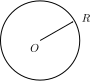
\includegraphics{figWarm1.pdf}		
\end{wrapfigure}
Будем искать решение в виде функции 
\[
	u = X(p)\cdot Y(t)
\]
Подставляем в уравнение
\[ 
	X(p)Y'(t) = Y(t) X''(p) +\frac{1}{p} Y(t) X'(p)
\]
Получаем следующее соотношение
\[
	\frac{Y'(t)}{Y(t)} = \frac{X''(p) + \frac{1}{p} X'(p)}{X(p)} = - k^2
\]
Для $X$ получаем дифференциальное уравнение 2-го порядка
\[
	X'' + \frac{1}{p} X' +k^2 X = 0
\]
Сделаем замену $\xi = k p$
\[
	  \der{X}{\xi}{2} + \frac{1}{\xi} \der{X}{\xi}{} + X = 0
\]
Будем искать решение в виде 
\[
	X(\xi) = \sum\limits_{k = 0}^{\infty} a_k \xi^k
\]
Находим первые две производные
\begin{align*}
	&X'(\xi)= \sum\limits_{k = 1}^{\infty} a_k k \xi^{k - 1}\\
	&X''(\xi) =  \sum\limits_{k = 2}^{\infty} a_k (k - 1) k \xi^{k - 2}
\end{align*}
и подставляем в полученное уравнение 
\[
	a_0 + a_1 \xi + a_1 \frac{1}{\xi} + \sum\limits_{k = 2}^{\infty} (a_k (k - 1) k \xi^{k - 2} + a_k k \xi^{k - 2} + a_k \xi^k) = 0 
\]
Приравнивая коэффициенты при соответствующих степенях $\xi$, находим $a_i$
\[
	\frac{1}{\xi} a_1 = 0 \quad \xi^0: a_0 + 4 a_2 = 0
\]

\[
	\xi^1 a_1 + 3 a_3 + 6 a_3 = 0 \Rightarrow  a_{2k + 1} = 0 \quad k \in N \cup {0}
\]
Получаем
\[
	X(p) = \sum (-1)^n \frac{\xi^{2n}}{2^{2n} (n!)^2}
\]~--функция Бесселя нулевого порядка.\\

Исследуем ряд на сходимость:\\
Достаточно показать, что n-ый член (при $n \rightarrow \infty$) стремится к 0.\\
	\[X(p) = I_0 (k p) = \sum (-1)^n \frac{(k p)^2n}{2^{2n} (n!)^2}\]

В итоге получаем
\[u_n(p, t) = c_n e^{- k_n^2 t} J_0 (k_n p)\]
Решение исходной задачи будет представляться в таком виде
\[u(p, t) = \sum\limits_{n = 0}^{\infty} u_n (p, t) = \sum\limits_{n = 0}^{\infty} C_n e^{- k_n^2 t} J_0(k_n p)\]
Определим $k_n$: $u(R, 0) = 0 \Rightarrow J_0(k_n R) = 0$\\
Уравнение решается и имеет счётное количество корней - $k_n$.

\[
	t=0 \quad u(\rho, 0) = \varphi(\rho ) = \sum\limits_{n =0 }^{\infty} C_n J_0 (k_n \rho) e^0
\]

Для функции Бесселя:\\ 
	\[\int\limits_0^R J_0 (k_n p) I_0(k_m p) p dp = \begin{cases} \frac{1}{2} {J_0'}^2 (k_n R) & k=m \\ 0 & k \neq m \end{cases}\]

Это свойство можно использовать для нахождения коэффициентов $C_n$ следующим образом
\[
	\int\limits_0^R\rho\varphi(\rho) J_0(k_N \rho) d\rho = C_n \int_0^R \rho J_0^2 (k_n \rho) d \rho
\]
\[
	C_n =\frac{\int\limits_0^R \rho \varphi(\rho) J_0 (k_n \rho) d \rho}{\int\limits_0^R \rho J_0^2 (k_n\rho) d\rho}
	\]